% !TeX root=SBUKThesis-main.tex
\chapter{نتایج و بحث}\label{chap4}
\section{مجموعه داده های مورد استفاده}

روش مولد اعلان ساده را در مجموعه‌ای گسترده از وظایف مرتبط با استدلال حسابی
\LTRfootnote{arithmetic reasoning}
 و استدلال مبتنی بر درک مسئله
 \LTRfootnote{commonsense reasoning}
  مورد ارزیابی قرار داده\/ایم. برای این منظور از هشت مجموعه داده‌ی عمومی، شامل 
  GSM8K \cite{GSM8k}
   ،
  SVAMP \cite{SVAMP}
   ،
  MultiArith \cite{MultiArith}
   ،
  AddSub \cite{AddSub}
   ،
  AQuA-RAT \cite{AquaRat}
   و
  SingleEq \cite{SingleEQ}
  
   به همراه CommonsenseQA \cite{CSQA} و StrategyQA \cite{SQA} استفاده شده است.
   
همانطور که در جدول \ref{tab_Results} می\/بینید، روش مولد اعلان ساده با روش‌های زنجیره تفکر، برنامه\/ریزی و حل با اعلان بهبود یافته و بدون آن، مهندس اعلان خودکار و بهینه\/سازی با اعلان ها مورد مقایسه قرار گرفته است. بالاترین دقت برای هر مجموعه داده به صورت فونت برجسته مشخص شده است. نتایج مدل زبان text-davinci-003 مستقیماً از مقاله‌ی برنامه\/ریزی و حل \cite{PS} استخراج شده و نتایج مدل زبان PaLM 2-L نیز به طور مستقیم از مقاله‌ی مولد اعلان \cite{PromptBreeder} گرفته شده‌اند. جهت تضمین مقایسه‌ای عادلانه، تمامی روش ها با مدل زبانی Mistral ارزیابی شده\/اند و سپس نتایج مقایسه شده است.

\begin{table}[h!]
		\centering
		{\resizebox{\textwidth}{!}{%
			\begin{LTR} % Begin left-to-right environment
			\begin{tabular}{c|ll|ccccccccc}
				\textbf{Results from} &\textbf{Method}  &\textbf{LLM}  & MultiArith  &SingleEq  &AddSub  &SVAMP  &SQA  &CSQA  &AQuA-RAT &GSM8K \\\hline
				\multirow{4}{*}{PS \cite{PS}}
				&COT  &text-davinci &\lr{83.8}  &\lr{88.1}  &\lr{85.3}  &\lr{69.9}  &\lr{63.8}  &\lr{65.2}  &\lr{38.9}  &\lr{56.4} \\
				&POT &text-davinci &\lr{92.2}  &\lr{91.7}  &\lr{85.1}  &\lr{70.8}  &-  &-  &\lr{43.9}  &\lr{57.0} \\
				&PS &text-davinci &\lr{87.2}  &\lr{89.2}  &\lr{88.1}  &\lr{72.0}  &-  &-  &\lr{42.5}  &\lr{58.2} \\
				&PS+ &text-davinci &\lr{91.8}  &\lr{94.7}  &\lr{92.2}  &\lr{75.7}  &\lr{65.4}  &\lr{71.9}  &\lr{46.0}  &\lr{59.3} \\\hline
				\multirow{5}{*}{PB\cite{PromptBreeder}}
				&PS &PaLM 2-L  &\lr{97.7}  &\lr{90.6}  &\lr{72.4}  &\lr{83.8}  &\lr{50.0}  &\lr{77.9}  &\lr{40.2}  &\lr{59.0} \\
				&PS+ &PaLM 2-L  &\lr{92.5}  &\lr{94.7}  &\lr{74.4}  &\lr{86.3}  &\lr{50.1}  &\lr{73.3}  &\lr{39.4}  &\lr{60.5} \\
				&APE &PaLM 2-L  &\lr{95.8}  &\lr{82.2}  &\lr{72.2}  &\lr{73.0}  &\lr{38.4}  &\lr{67.3}  &\lr{45.7}  &\lr{77.9} \\
				&OPRO &PaLM 2-L  &-  &-  &-  &-  &-  &-  &-  &80.2 \\
				&PB &PaLM 2-L  &\textbf{\lr{99.7}}  &\textbf{\lr{96.4}}  &\lr{87.8}  &\lr{90.2}  &\lr{71.8}  &\lr{85.4}  &\lr{62.2}  &\lr{83.9} \\\hline
				\multirow{6}{*}{\text{مولد اعلان ساده(us)}}
				&CoT &Mistral  &\lr{79.0}  &\lr{85.0}  &\lr{78.0}  &\lr{64.0}  &\lr{54.0}  &\lr{51.0}  &\lr{33.0}  &\lr{72.0} \\
				&PS &Mistral  &\lr{68.0}  &\lr{91.0}  &\lr{78.0}  &\lr{68.0}  &\lr{61.0}  &\lr{43.0}  &\lr{36.0}  &\lr{66.0} \\
				&PS+ &Mistral  &\lr{82.0}  &\lr{84.0}  &\lr{80.0}  &\lr{62.0}  &\lr{44.0}  &\lr{27.0}  &\lr{26.0}  &\lr{60.0} \\
				&APE &Mistral  &\lr{78.0}  &\lr{86.0}  &\lr{84.0}  &\lr{69.0}  &\lr{54.0 } &\lr{51.0}  &\lr{36.0}  &\lr{66.0} \\
				&OPRO &Mistral  &\lr{85.0}  &\lr{84.0}  &\lr{78.0}  &\lr{61.0}  &\lr{53.0}  &\lr{35.0}  &\lr{34.0}  &\lr{67.0} \\
				&مولد اعلان ساده(ours) &Mistral  &\cellcolor{mybluecolor!20}\lr{92.0 } &\cellcolor{mybluecolor!60}\lr{94.0 } &\cellcolor{mybluecolor!90}\textbf{\lr{89.0}}  &\cellcolor{mybluecolor!90}\textbf{\lr{93.0}}  &\cellcolor{mybluecolor!90}\textbf{\lr{92.0}}  &\cellcolor{mybluecolor!90}\textbf{\lr{91.0}}  &\cellcolor{mybluecolor!90}\textbf{\lr{93.0}}  &\cellcolor{mybluecolor!90}\textbf{\lr{84.0}} \\\hline
			\end{tabular}
		\end{LTR}
	}
		}
		\caption{مقایسه دقت روش مولد اعلان ساده با سایر روش های موجود} 
		\label{tab_Results}
	 % End left-to-right environment
\end{table}

\section{متغیرهای روش مولد اعلان ساده}
 از آن‌جایی که مولد اعلان ساده یک الگوریتم تکاملی است، این الگوریتم را در بازه ۲۰ تا ۳۰ تکرار
 \LTRfootnote{Epoch}
  اجرا می‌کنیم؛ تا جایی ‌که در آخرین تکرار‌ها، مجموعه کاندیدا تغییر نخواهد کرد. در هر دوره، جمعیتی متشکل از ۱۲۰ تا ۱۵۰ اعلان دستوری، بسته به مجموعه کاندیدا، تولید می‌شود. همانطور که در فصل قبل گفته شد، این اعلان‌ها بر اساس توضیحات مسئله و یک مجموعه آموزشی شامل ۲۰ سوال و پاسخ از مجموعه داده، نمونه‌گیری می‌شوند. از میان این جمعیت، زیرمجموعه‌ای شامل ۱۰ اعلان دستوری انتخاب شده و بر روی یک مجموعه اعتبارسنجی که شامل ۲۰ سوال و پاسخ متمایز از مجموعه آموزشی است، ارزیابی می‌گردد.

\noindent پس از اتمام تمامی دوره‌ها، اعلان‌های دستوری با بهترین عملکرد بر روی مجموعه‌ای شامل ۱۰۰  سوال و پاسخ که به‌طور تصادفی از مجموعه داده انتخاب شده و از هر دو مجموعه آموزشی و اعتبارسنجی متمایز می‌باشند، مورد آزمون قرار می‌گیرند.

\noindent
 پارامتر توضیحات مسئله به مجموعه داده بستگی دارد که در جدول \ref{tab_des} توضیح متناظر با هر مجموعه داده آورده شده است.
 
 در این پژوهش، از مدل زبانی Mistral-7B \cite{mistral} برای تولید و آزمون اعلان‌های دستوری استفاده می‌شود. همچنین، به منظور تبدیل اعلان‌های دستوری به بردار عددی، از مدل تبدیل جمله‌ی
 \LTRfootnote{Sentence Embedding}
 \lr{bert-base-nli-mean-tokens}
   موجود در سایت HuggingFace بهره گرفته شده است.
   
   
\section{روش های مرجع}
    نتایج روش مولد اعلان ساده با استفاده از پیشرفته‌ترین روش‌های مهندسی که در فصل های قبلی به تفصیل توضیح داده شده اند، مورد مقایسه قرار گرفته‌اند. به‌منظور تضمین مقایسه‌ای عادلانه، در صورت امکان، این روش‌ها با استفاده از مدل پایه Mistral مجدداً اجرا شده‌اند زیرا امکان اجرای روش مولد اعلان ساده با مدل های text-davinci-003 و PaLM 2-L  وجود ندارد چرا که این مدل‌ها به صورت عمومی در دسترس نمی‌باشند و روش های دسترسی به آن‌ها منسوخ شده است. اعلان‌های دستوری این روش‌ها به‌طور مستقیم از مقاله مولد اعلان استخراج شده‌اند؛ اما اعلان‌های تولید شده توسط مولد اعلان مورد آزمون قرار نگرفته‌اند زیرا آن‌ها به‌گونه‌ای برای PaLM 2 بهینه‌سازی شده‌اند که استفاده از آن‌ها در مدل Mistral مقایسه‌ای منصفانه ارائه نخواهد داد.
   
لازم به یادآوری است که برای هر مجموعه داده و هر روش، از دقت به عنوان معیار ارزیابی استفاده شده است.
     
\section{نمایش دوبعدی اعلان ها}
برای درک بهتر عملکرد مدل احتمالاتی فرآیندهای نقطه\/ای دترمینانی در طول تکرارها، در شکل \ref{fig_visualize-dpp} توزیع دو بعدی بردار های عددی اعلان ها را نمایش داده‌ایم.
برای کاهش ابعاد این  بردار های عددی، ابتدا از روش کاهش بعد PCA \cite{pca} برای کاهش ابعاد به ۵۰ و سپس از روش t-SNE \cite{tsne} برای کاهش 50 بعد به ۲ بعد استفاده کردیم.
همانطور که دیده می\/شود، توزیع یکنواخت دستورالعمل‌های انتخاب‌شده در نواحی مختلف فضای جستجو نمایش داده شده است که بیانگر توازن میان تنوع و کیفیت در این روش است.

\begin{figure}[!ht]
	\centering
	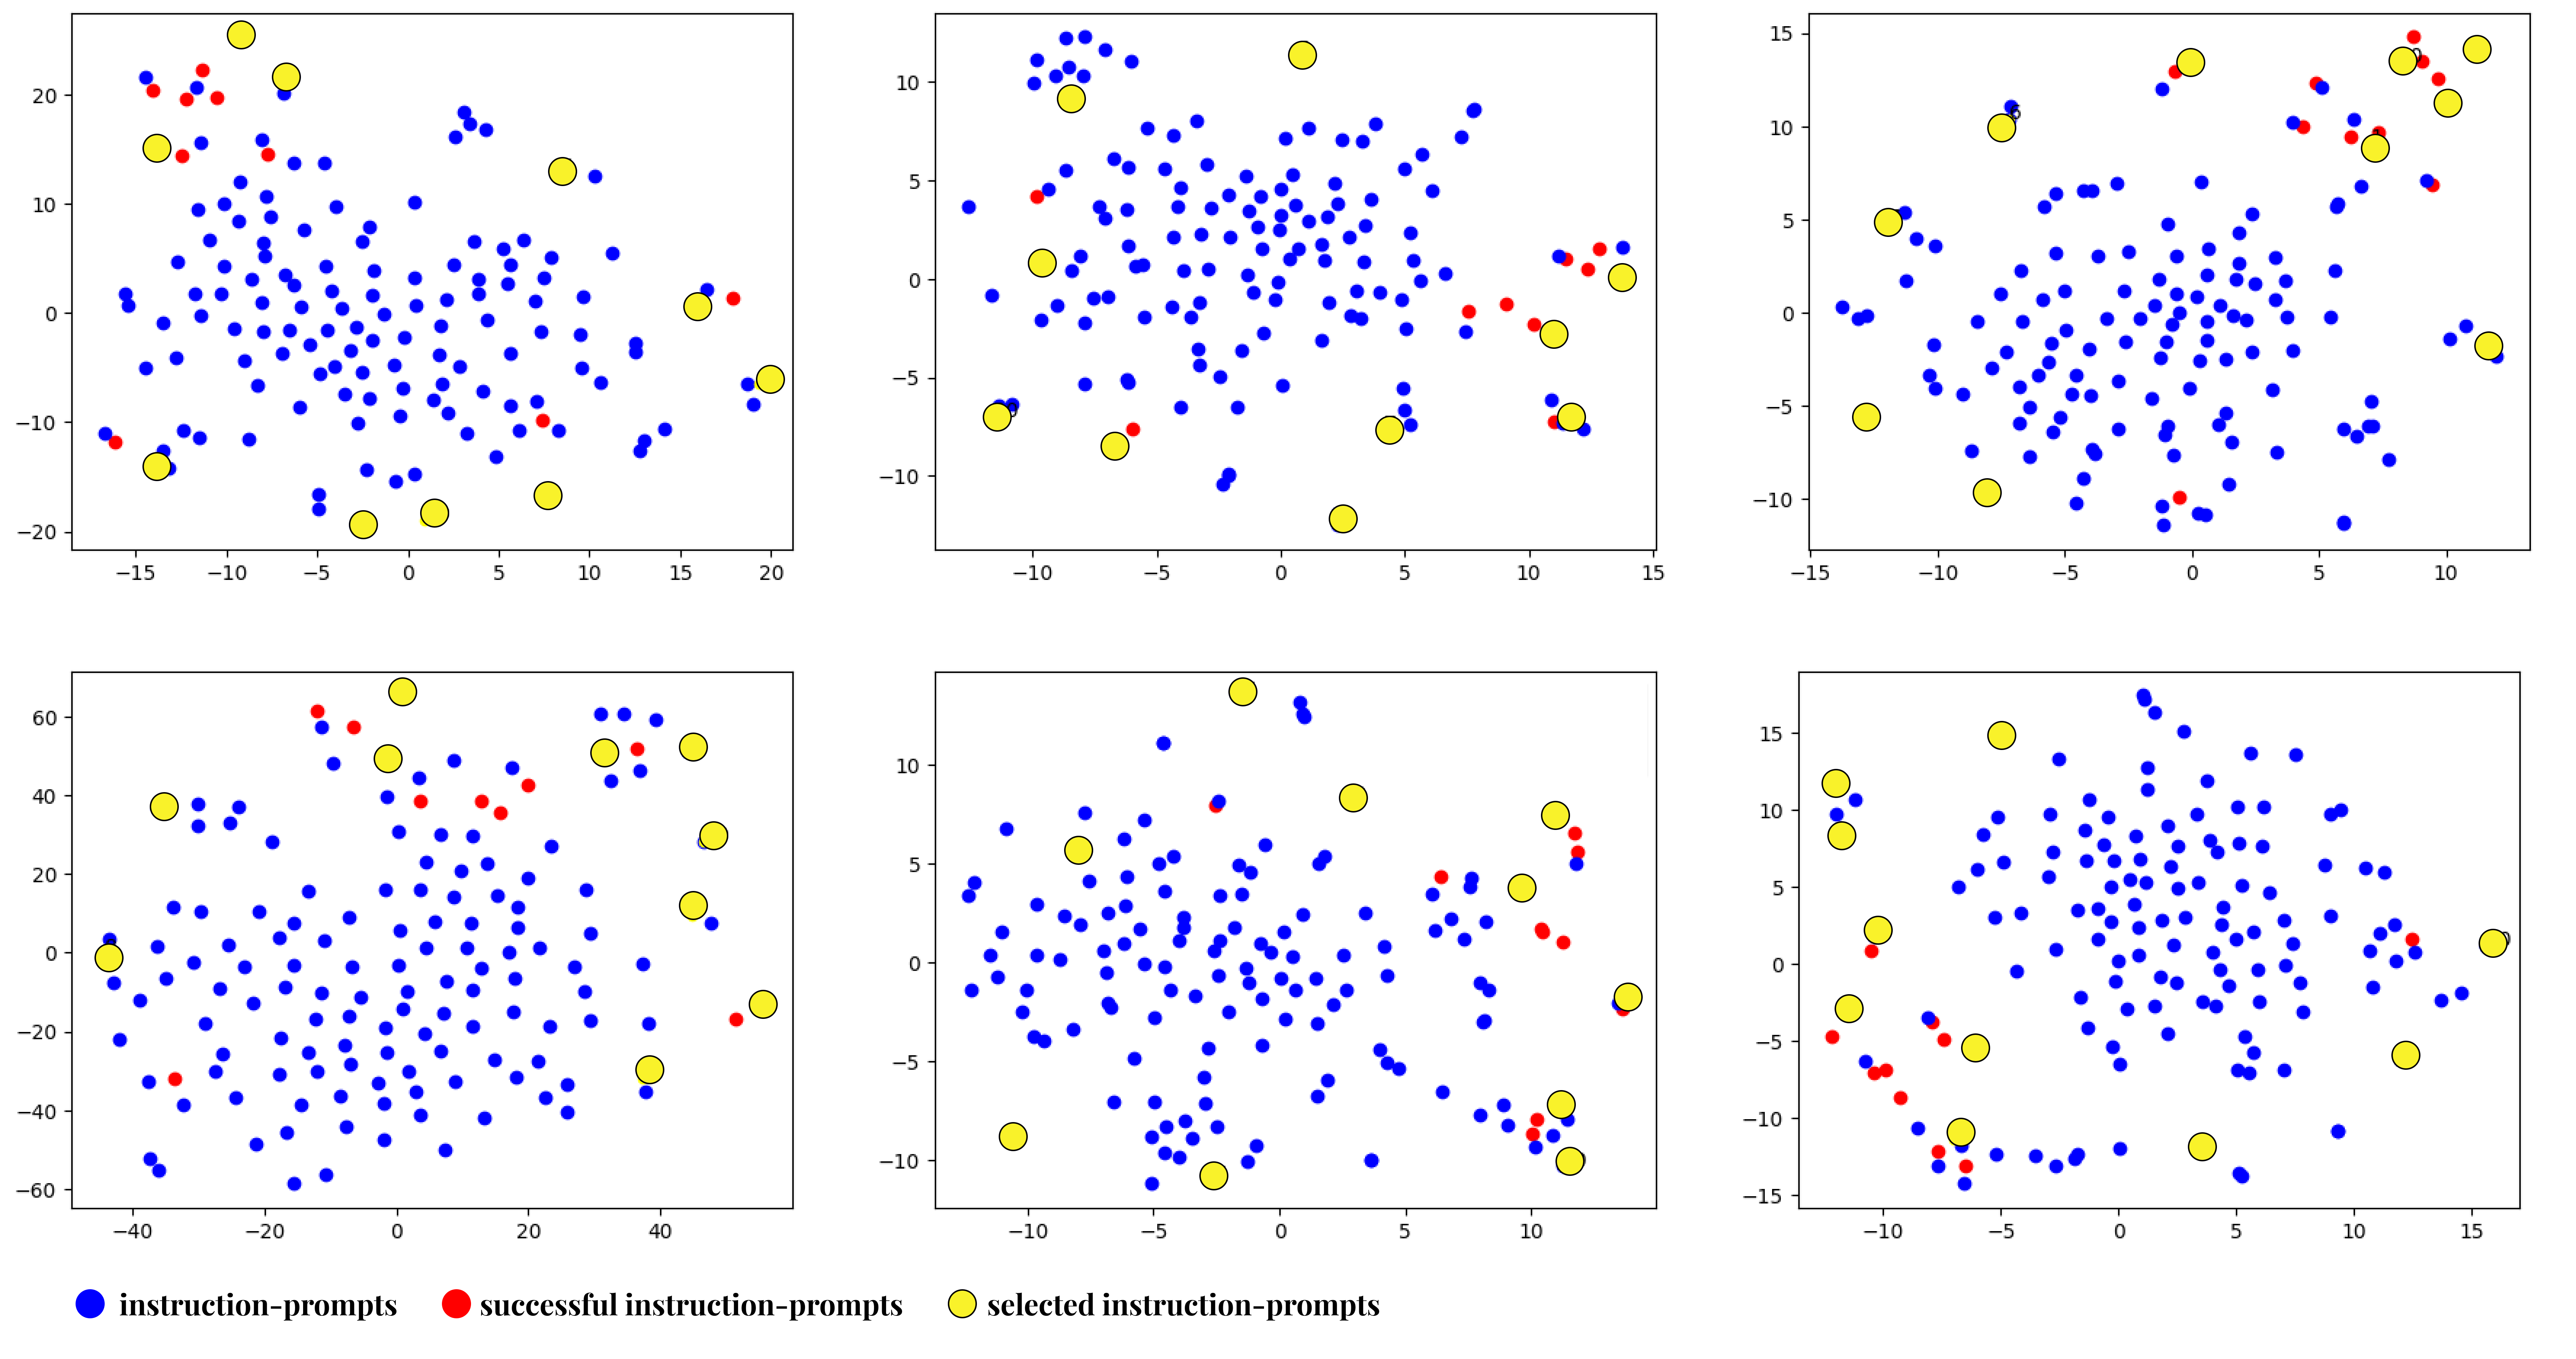
\includegraphics[width=140mm]{images/eval}
	\caption{نمایش دو بعدی بردار اعلان ها برای ارزیابی انتخاب در روش مولد اعلان ساده}
	\label{fig_visualize-dpp}
\end{figure}

     
\section{نتایج}
نتایج اجرای روش مولد اعلان ساده بر روی مجموعه داده‌های مذکور نشان می‌دهد که این روش از پیشرفته‌ترین روش‌های مهندسی برتری دارد. همانطور که در جدول \ref{tab_Results} مشاهده می‌شود، مولد اعلان ساده در تمامی مجموعه داده‌ها از سایر روش ها برتر است.

ابتدا عملکرد هر روش را در میان مدل‌های زبانی مختلف ارزیابی کردیم. مشاهده می‌شود که اکثر روش‌ها دقت مشابهی در میان مدل‌های مختلف دارند، اگرچه بهبودهایی در عملکرد هنگام تغییر از 
\lr{text-davinci-003 }
به 
\lr{PaLM 2-L} 
و از 
\lr{PaLM 2-L}
 به 
\lr{Mistral}
  دیده می‌شود؛ این بهبودها را می‌توان به پیشرفت‌های موجود در دقت و ساختار مدل‌های زبانی نسبت داد. 

برای تضمین صحت مقایسه، از روش برنامه\/ریزی و حل به عنوان نقطه مرجع استفاده شده و بهبود نسبی مولد اعلان و مولد اعلان ساده محاسبه گردیده است. در روش مولد اعلان، با استفاده از فرمول زیر به بهبود نسبی
 \lr{23.4 ٪}
  نسبت به روش برنامه\/ریزی و حل در میان مجموعه داده‌ها دست یافتیم:

\[
\begin{split}
	\text{بهبود نسبی مولد اعلان} = \frac{1}{8} \Bigg[
	& \frac{99.7}{97.7} + \frac{96.4}{90.6} + \frac{87.8}{72.4}  + \frac{90.2}{83.8} \\
	& + \frac{71.8}{50.0} + \frac{85.4}{77.9} + \frac{62.2}{40.2} + \frac{83.9}{59.0}
	\Bigg],
\end{split}
\]
در همین حال، برای مولد اعلان ساده با فرمول زیر، به بهبود نسبی
\lr{54.7 ٪} 
 نسبت به روش برنامه\/ریزی و حل در میان مجموعه داده‌ها دست یافتیم:

     
\[
 \begin{split}
   	\text{بهبود نسبی مولد اعلان ساده} = \frac{1}{8} \Bigg[
   	& \frac{92.0}{68.0} + \frac{94.0}{91.0} + \frac{89.0}{78.0} + \frac{93.0}{68.0}\\
   	& + \frac{92.0}{61.0} + \frac{91.0}{43.0}  + \frac{93.0}{36.0} + \frac{84.0}{66.0}
   	\Bigg],
 \end{split}
\]
     
     
\section{سربار محاسباتی}
همانطور که در بخش پارامتر های روش مولد اعلان ساده توضیح داده شد، مولد اعلان ساده به‌طور مشابه با مولد اعلان در بازه ۲۰ تا ۳۰ تکرار اجرا می‌شود. در هر تکرار، مولد اعلان ساده جمعیتی متشکل از ۱۰۰ تا ۱۲۰ اعلان دستوری تولید می‌کند که برای هر یک، یک فراخوانی مدل زبانی مورد نیاز است. در مقابل، مولد اعلان با جمعیتی متشکل از ۵۰ واحد عمل می‌کند؛ هر واحد شامل یک جفت اعلان است که منجر به ۱۰۰ فراخوانی مدل زبانی برای تولید آن‌ها می‌شود. در گام بعدی، برای انتخاب و جهش، مولد اعلان از رویکرد ترکیبی جهش و ابرجهش استفاده می‌کند که برای هر آیتم از واحدهای جمعیت، حداقل دو فراخوانی مدل زبانی نیاز دارد. بنابراین، تعداد کل فراخوانی‌های مدل زبانی در این مرحله برای مولد اعلان به صورت زیر محاسبه می‌شود:
\[
50 \times 2 \times 2 = 200.
\]
در مقابل، مولد اعلان ساده این محاسبات را با استفاده از محاسبات روش DPP انجام می‌دهد و از فراخوانی‌های اضافی مدل زبانی در این گام صرف نظر می‌کند.

در انتها، در گام ارزیابی، مولد اعلان کل جمعیت را مورد ارزیابی قرار داده و به هر واحد نمره می‌دهد. از آنجا که هر واحد در جمعیت مولد اعلان شامل یک جفت اعلان است، ارزیابی ۵۰ واحد نیازمند:
\[
50 \times 2 = 100
\]
فراخوانی مدل زبانی می‌باشد. اما مولد اعلان ساده تنها ۱۰ اعلان دستوری از میان ۱۰۰ اعلان برای ارزیابی انتخاب می‌کند و هر اعلان یک فراخوانی مدل زبانی نیاز دارد؛ بنابراین:
\[
10 \times 1 = 10.
\]
از سوی دیگر، اندازه‌ی مجموعه داده اعتبارسنجی برای مولد اعلان شامل ۱۰۰ جفت سوال و پاسخ است، در حالی که برای مولد اعلان ساده به ۲۰ کاهش یافته است. علاوه بر این، مولد اعلان ساده پس از شناسایی اعلان‌های با عملکرد برتر، گام آزمون را به منظور تضمین مقایسه‌ای منصفانه اضافه می‌کند؛ این گام اعلان‌های انتخاب‌شده را بر روی مجموعه داده‌ای شامل ۱۰۰ جفت سوال و پاسخ مانند مولد اعلان ارزیابی می‌کند.

\noindent تعداد کل فراخوانی‌های مدل زبانی برای مولد اعلان و مولد اعلان ساده در هر دوره به صورت زیر بیان می‌شود:
\[
\text{کل فراخوانی‌های مدل زبانی برای مولد اعلان} = 100 + 200 + 100 = 400,
\]
\[
\text{کل فراخوانی‌های مدل زبانی برای مولد اعلان ساده} = 100 \text{ تا } 120 + 10 = 110 \text{ تا } 130.
\]
بنابراین، مولد اعلان ساده سربار محاسباتی را تقریباً به میزان ۳ برابر کاهش می‌دهد.
    
    
\section{خروجی ها}
با بررسی خروجی های روش مولد اعلان ساده ، مشاهده شد که اعلان‌های دستوری با بهترین عملکرد برای هر مجموعه داده، در قالب چارچوبی صریح ساختاربندی شده‌اند. این چارچوب شامل چند بخش است: بخش اول، توضیح مفصل وظیفه می‌باشد که با دقت به تشریح آن می‌پردازد و در برخی موارد شامل دستورالعمل‌هایی است که جنبه‌های مختلف وظیفه را توضیح می‌دهند. بخش دوم این اعلان، مسیر حل مسئله با توضیحات گام به گام جهت رفع مشکلات موجود در حوزه مربوطه است. در مرحله بعد، تعدادی مثال ارائه شده است که به عنوان نمایش نمونه از مجموعه آموزشی با ارائه راه‌حل کامل و گام به گام، جهت هدایت روند تفکر مدل زبانی به کار رفته‌اند. 

برای مثال، اعلان دستوری با بهترین عملکرد برای مجموعه داده MultiArith، در ابتدا وظیفه را به‌طور کامل تعریف می‌کند، سپس پنج مثال به همراه راه‌حل کامل آن‌ها ارائه می‌دهد و در نهایت، دستورالعمل‌هایی برای حل مسائل در این حوزه بیان می‌نماید. متن کامل این اعلان دستوری در کادر \ref{p_MutiArith} آورده شده است.



\begin{tcolorbox}[breakable,colframe=mybluecolor!100, colback=mybluecolor!20, title=بهترین اعلان دستوری تولید شده برای مجموعه داده MultiArith] \label{p_MutiArith}
	\begin{LTR}
	\textbf{Task:} Analyze the given math problem, break down the information, and compute the answer step by step. Present the final answer as an Arabic number.
	
	\textbf{Examples:}
	\begin{enumerate}
		\item \lr{Understand that April makes \$9 for every rose she sells. Estimate how many roses April started with, then calculate how many roses she ended with, in order to figure out the revenue she generated.}
		\begin{itemize}
			\item Compute the difference between the number of roses April started with and the number of roses she ended with to find the quantity of roses April sold.
			\item Multiply the number of roses sold by the cost per rose to determine the earnings incurred.
		\end{itemize}
		
		\item \lr{Understand the scenario in which Megan prepared 68 cupcakes, and her brother, Todd, consumed 32 of them. Find out how many packages Megan can assemble with 6 cupcakes per package.}
		\begin{itemize}
			\item Subtract the number of cupcakes Todd consumed from the total number of cupcakes Megan prepared to determine the remaining amount of uneaten cupcakes.
			\item Divide the quantity of uneaten cupcakes by the number of cupcakes needed to make one package to find the number of packages Megan can assemble.
		\end{itemize}
		
		\item \lr{Identify the situation in which Katie organized and counted 9 albums with a consistent number of pictures in each album. Determine the number of pictures in each album.}
		\begin{itemize}
			\item Sum the total number of pictures Katie has to obtain the grand total.
			\item Divide the grand total by the number of albums to figure out the number of pictures in each album.
		\end{itemize}
		
		\item \lr{Grasp the details that Tiffany earns 6 points for each treasure she discovers. Figure out the point score Tiffany received from finding treasures on the first and second levels.}
		\begin{itemize}
			\item Add the number of treasures Tiffany discovered on the first and second levels to get the sum of treasures found.
			\item Multiply the total number of treasures by the points per treasure to learn the point score Tiffany attained.
		\end{itemize}
		
		\item \lr{Recall the situation in which a waiter manages 33 customers. Estimate how many customers the waiter is still serving after some prospective diners left and others joined the restaurant.}
		\begin{itemize}
			\item Subtract the number of customers who left from the current number of customers to determine the number of customers still at the restaurant.
			\item Add the number of new customers who arrived to find the updated number of customers the waiter is currently serving.
		\end{itemize}
	\end{enumerate}
	
	\textbf{Instructions:}
	\begin{enumerate}[label=\arabic*.]
		\item Explore the given problem to recognize the necessary computations needed to derive the solution.
		\item Break down the problem into more manageable parts for better organization and clarity.
		\item Calculate the solutions step by step.
		\item Deliver the numerical solution.
	\end{enumerate}
	\end{LTR}

\end{tcolorbox}
     
     
     
     
     
     
     
     
     
     
     
     